\bibliography{dissertation}
\appendix

\chapter{AI Usage}
\label{appx:ai_prompt}

I did not directly prompt any Large Language Models, or any other AI model, to assist with the writing of my dissertation or implementation. However, as listed in the Supporting Technologies list, I used GitHub Copilot to help with writing some tests for the parser and type checker. I used it via the VS Code extension, which uses the context of your file, to provide advanced AI autocompletion.

% =============================================================================

\chapter{Tokens for Lexical Analysis}
\label{appx:tokens}
Below is the code for how tokens outputted by lexical analysis are defined. 
\begin{lstlisting}
enum TokenType {
    EOF,
    Newline,

    Id,
    UppercaseId,

    If,
    Then,
    Else,

    Match,
    LBrace,
    RBrace,

    IntLit,
    FloatLit,
    StringLit,
    CharLit,
    BoolLit,

    DoubleColon,
    RArrow,
    Forall,
    KWType,
    KWData,

    LParen,
    RParen,

    Lambda,

    Dollar,
    Dot,
    Comma,
    Bar,

    Assignment,
}

struct Token {
    tt: TokenType,
    value: String,
}
\end{lstlisting}

\chapter{UI Screenshots}
\begin{figure}[h]
    \centering
    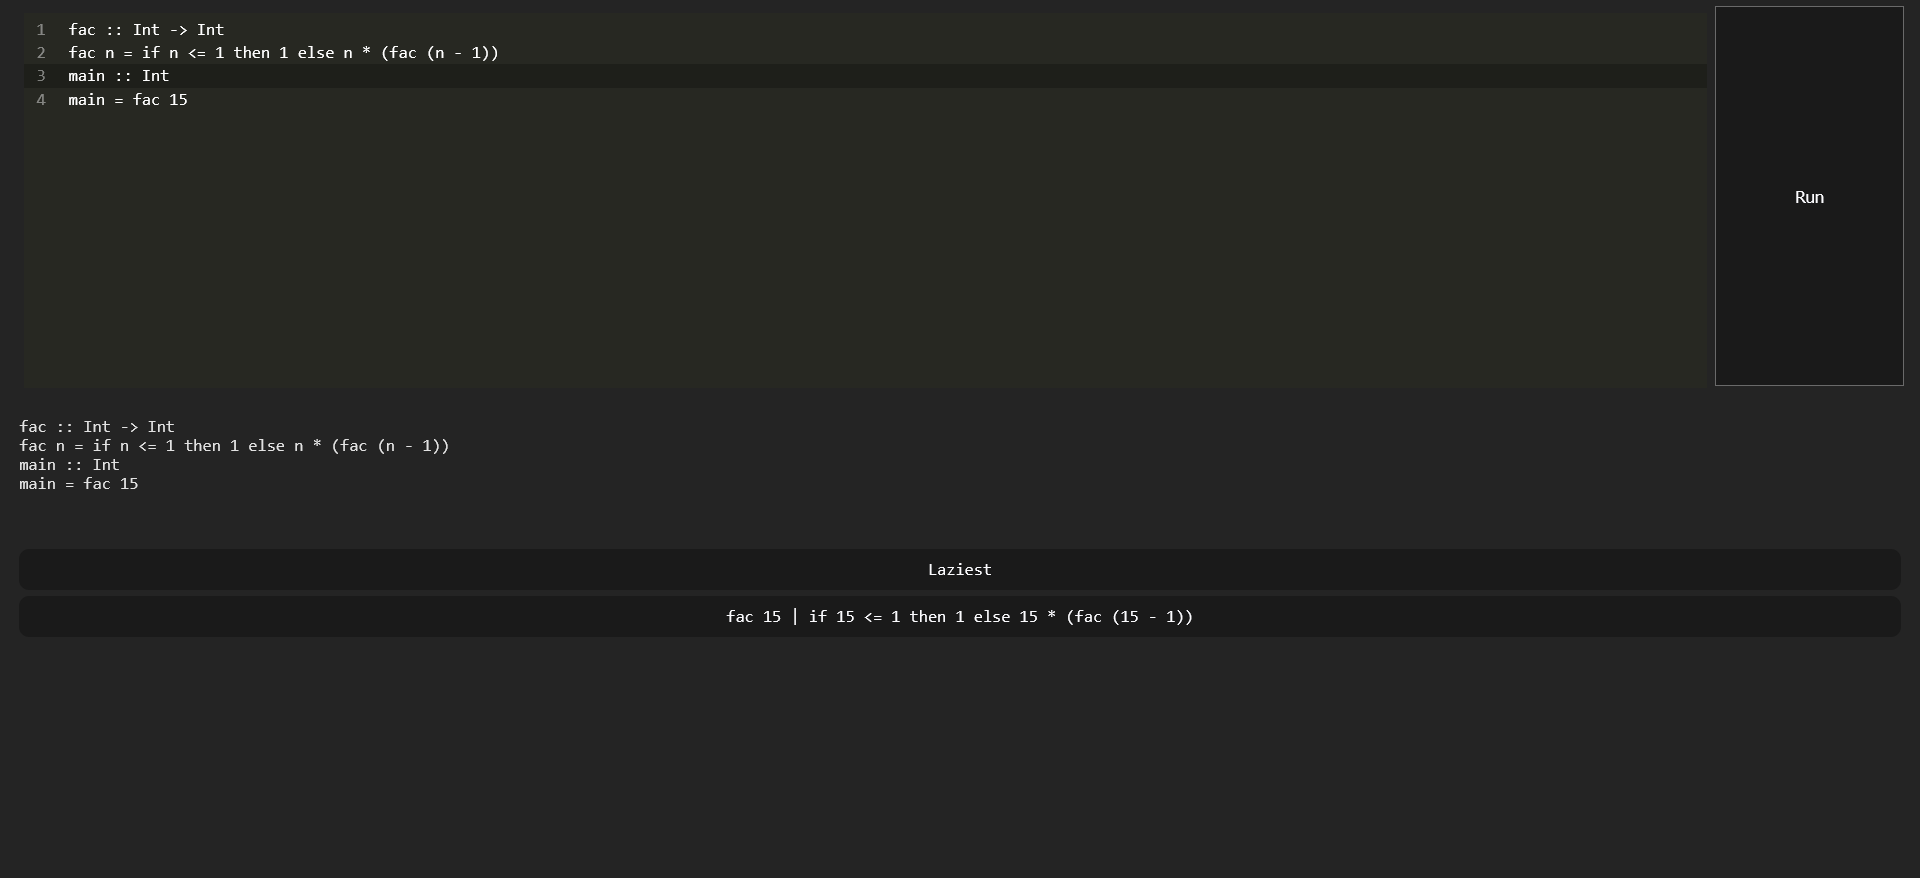
\includegraphics[width=1\linewidth]{images/cycle-1-end.png} 
    \captionsetup{justification=centering}
    \caption{The Web UI \ac{MVP}, as presented to my client at the end of cycle 1. Note that this does have type assignments, but these were just ignored by the parser and typechecker at this stage. }
    \label{fig:screenshot_cycle_1_end}
\end{figure}

\begin{figure}[h]
    \centering
    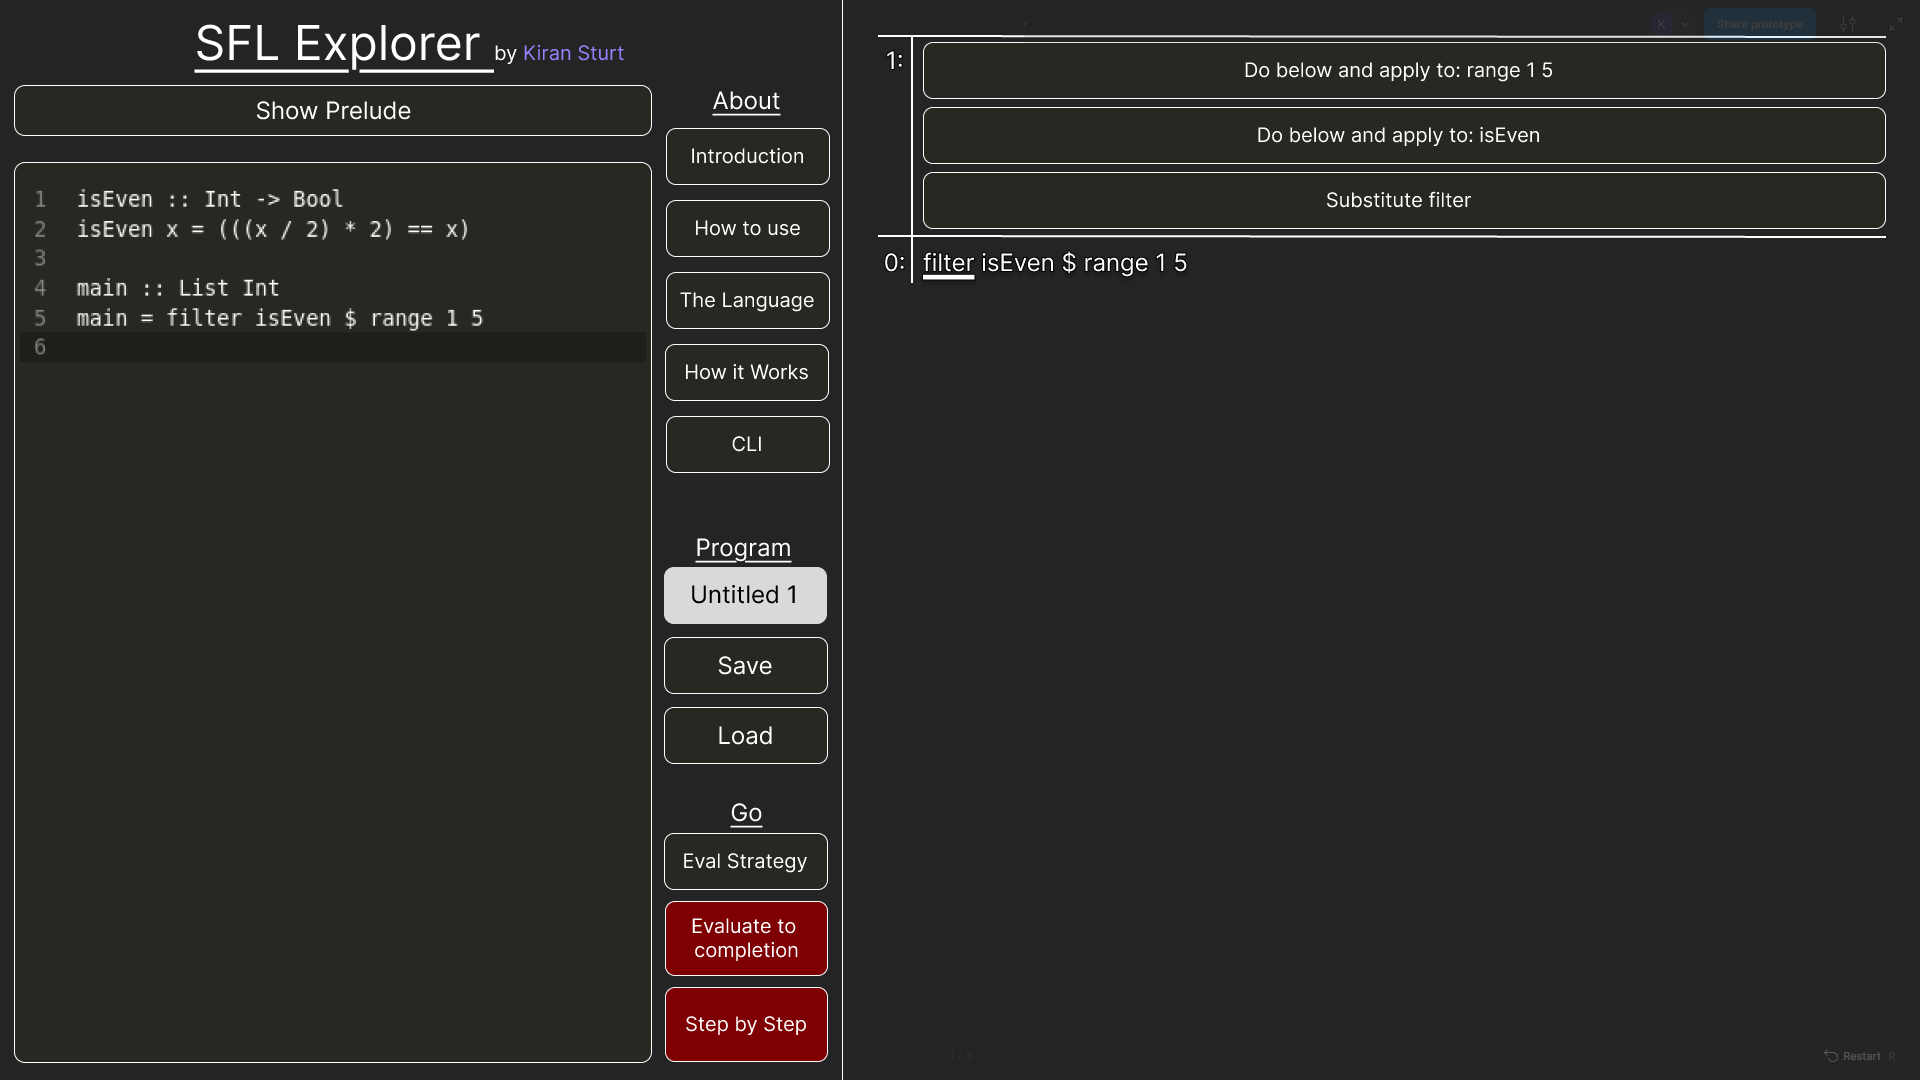
\includegraphics[width=1\linewidth]{images/figma_1.png} 
    \captionsetup{justification=centering}
    \caption{Screenshot 1 of the Figma design of the web UI}
    \label{fig:screenshot_figma1}
\end{figure}

\begin{figure}[h]
    \centering
    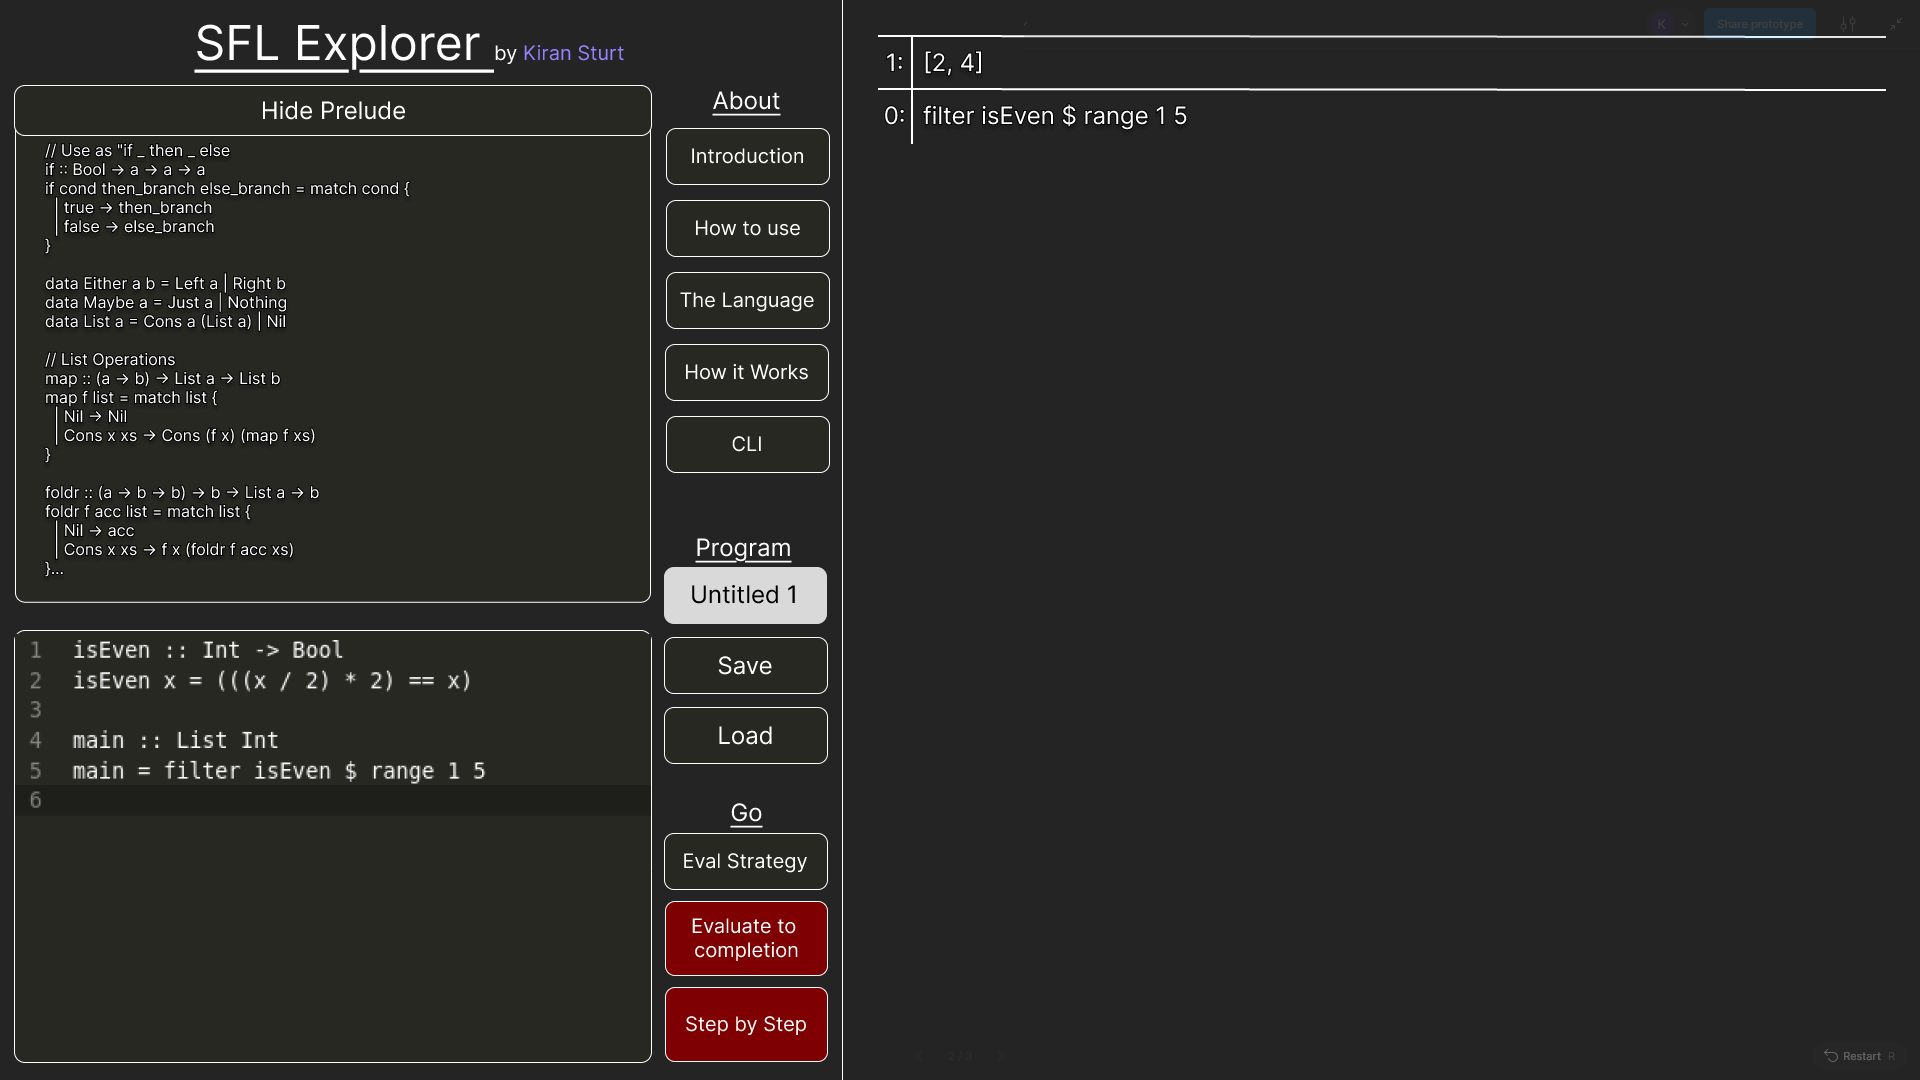
\includegraphics[width=1\linewidth]{images/figma_2.png}
    \captionsetup{justification=centering}
    \caption{Screenshot 2 of the Figma design of the web UI. This version shows the prelude extended}
    \label{fig:screenshot_figma2}
\end{figure}

\begin{figure}[h]
    \centering
    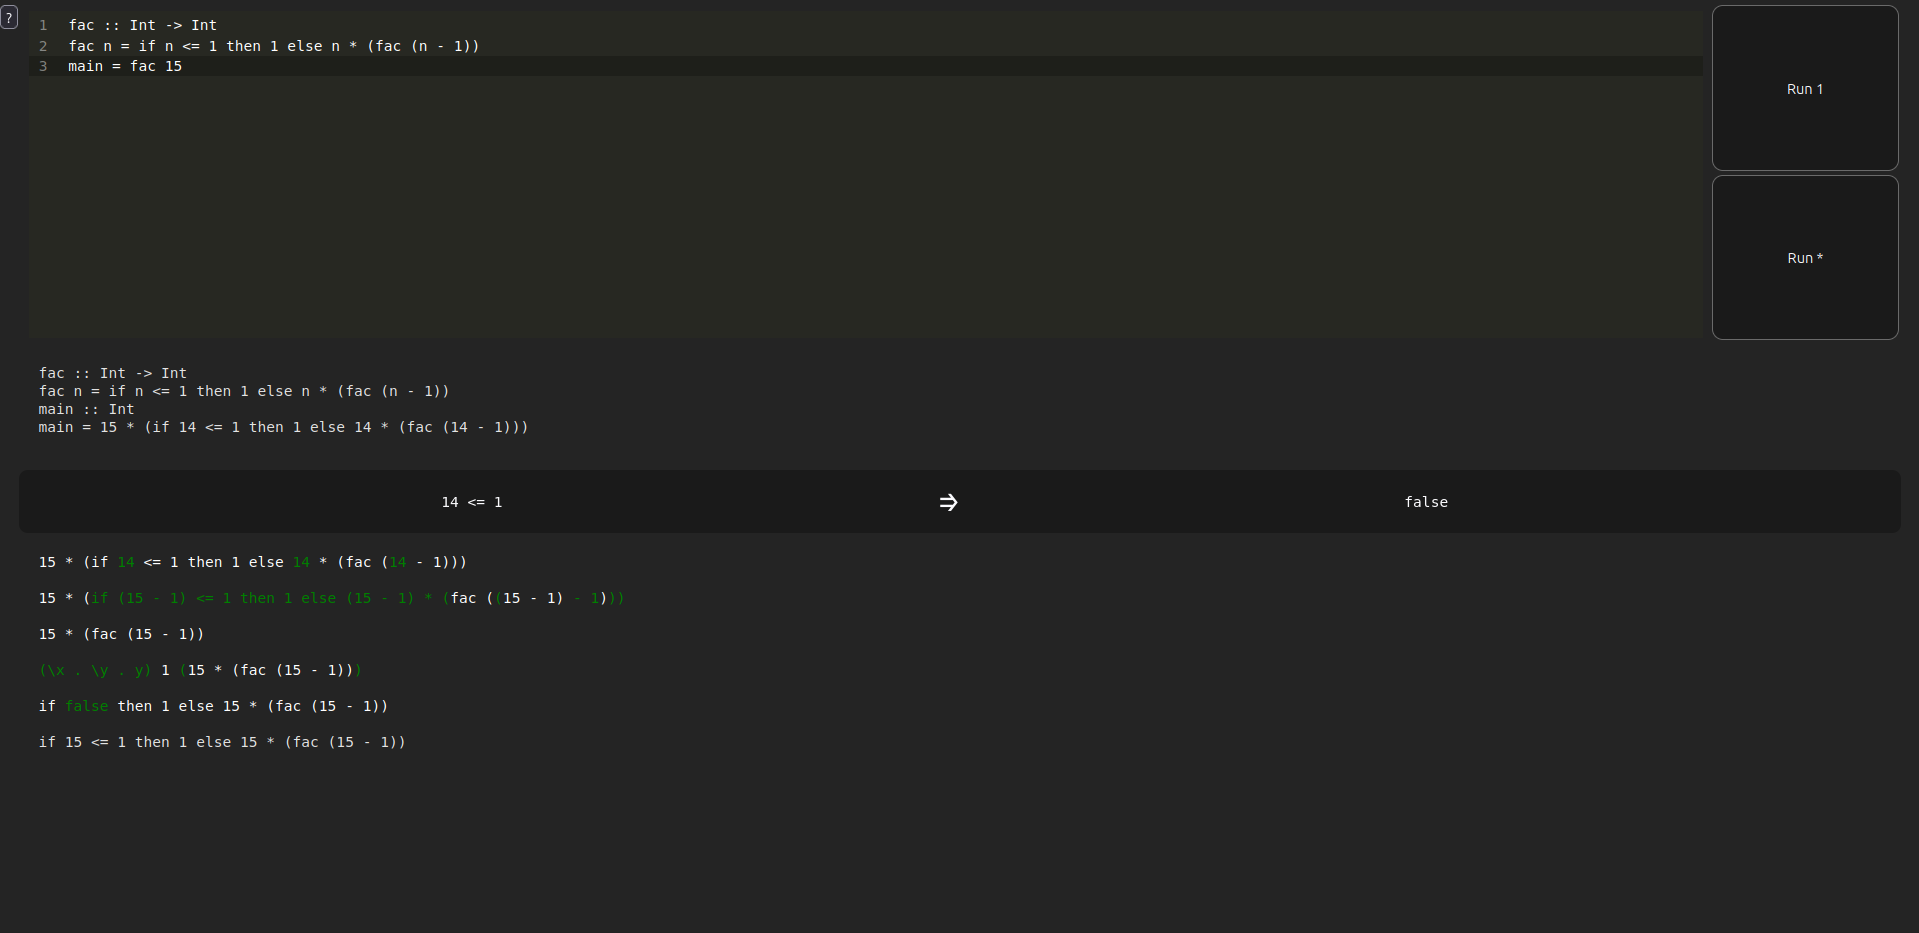
\includegraphics[width=1\linewidth]{images/product_at_testathon.png} 
    \captionsetup{justification=centering}
    \caption{The UI as tested in the testathon}
    \label{fig:screenshot_testathon}
\end{figure}

\begin{figure}[h]
    \centering
    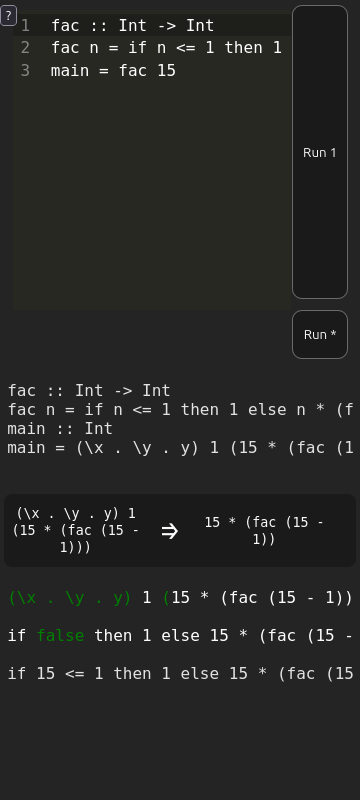
\includegraphics[width=0.3\linewidth]{images/testathon-mobile.png}
    \caption{The UI as tested in the testathon, as it would have appeared on a Samsung Galaxy S20}
    \label{fig:screenshot_testathon_mobile}
\end{figure}

\begin{figure}[h]
    \centering
    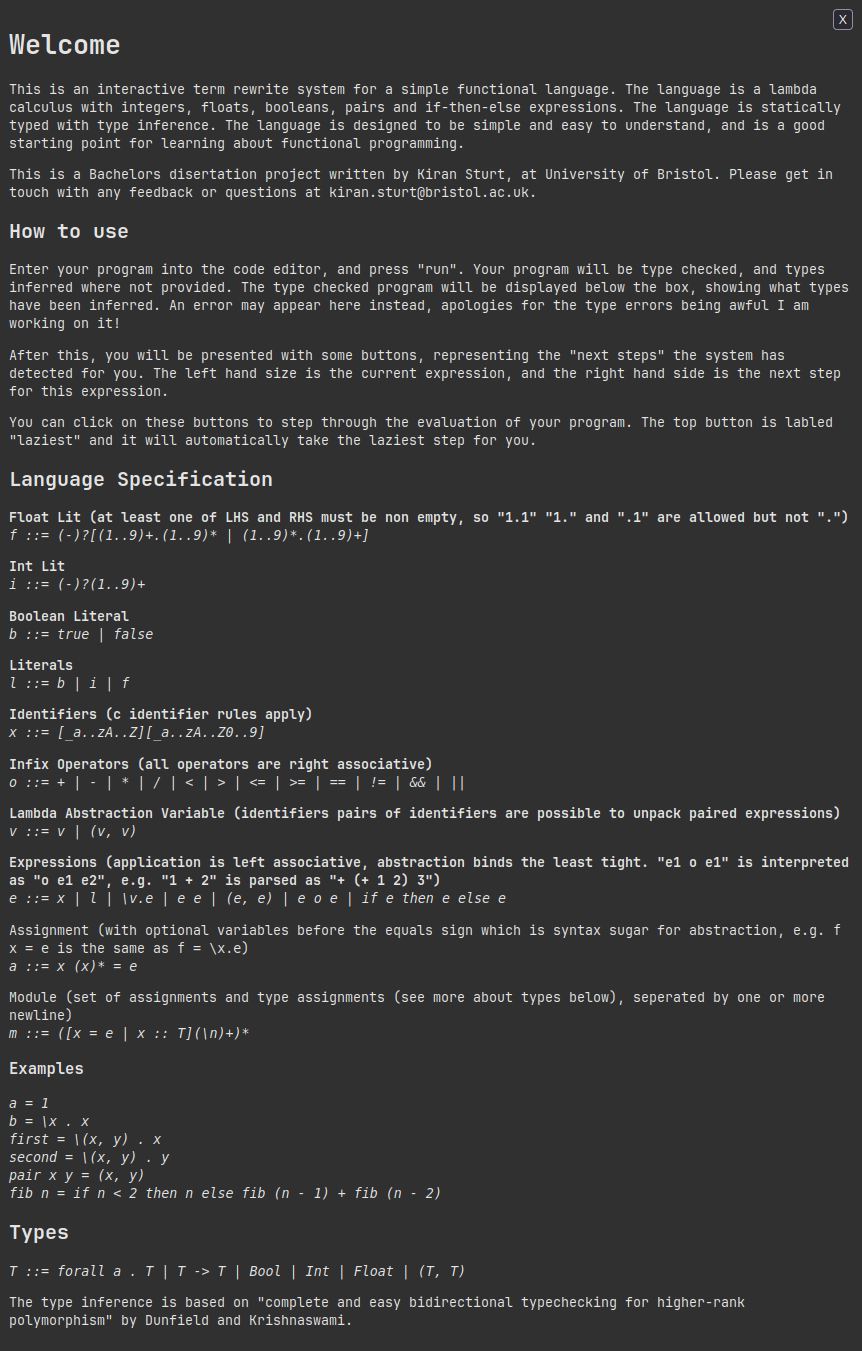
\includegraphics[width=0.9\linewidth]{images/testathon_help_menu_cropped.png} 
    \captionsetup{justification=centering}
    \caption{The "Help menu" in the testathon. This was spawned by pressing the "?" button in the top left of the UI, and dismissed by pressing the "X" button, or clicking outside of the box}
    \label{fig:screenshot_testathon_2}
\end{figure}

\begin{figure}[h]
    \centering
    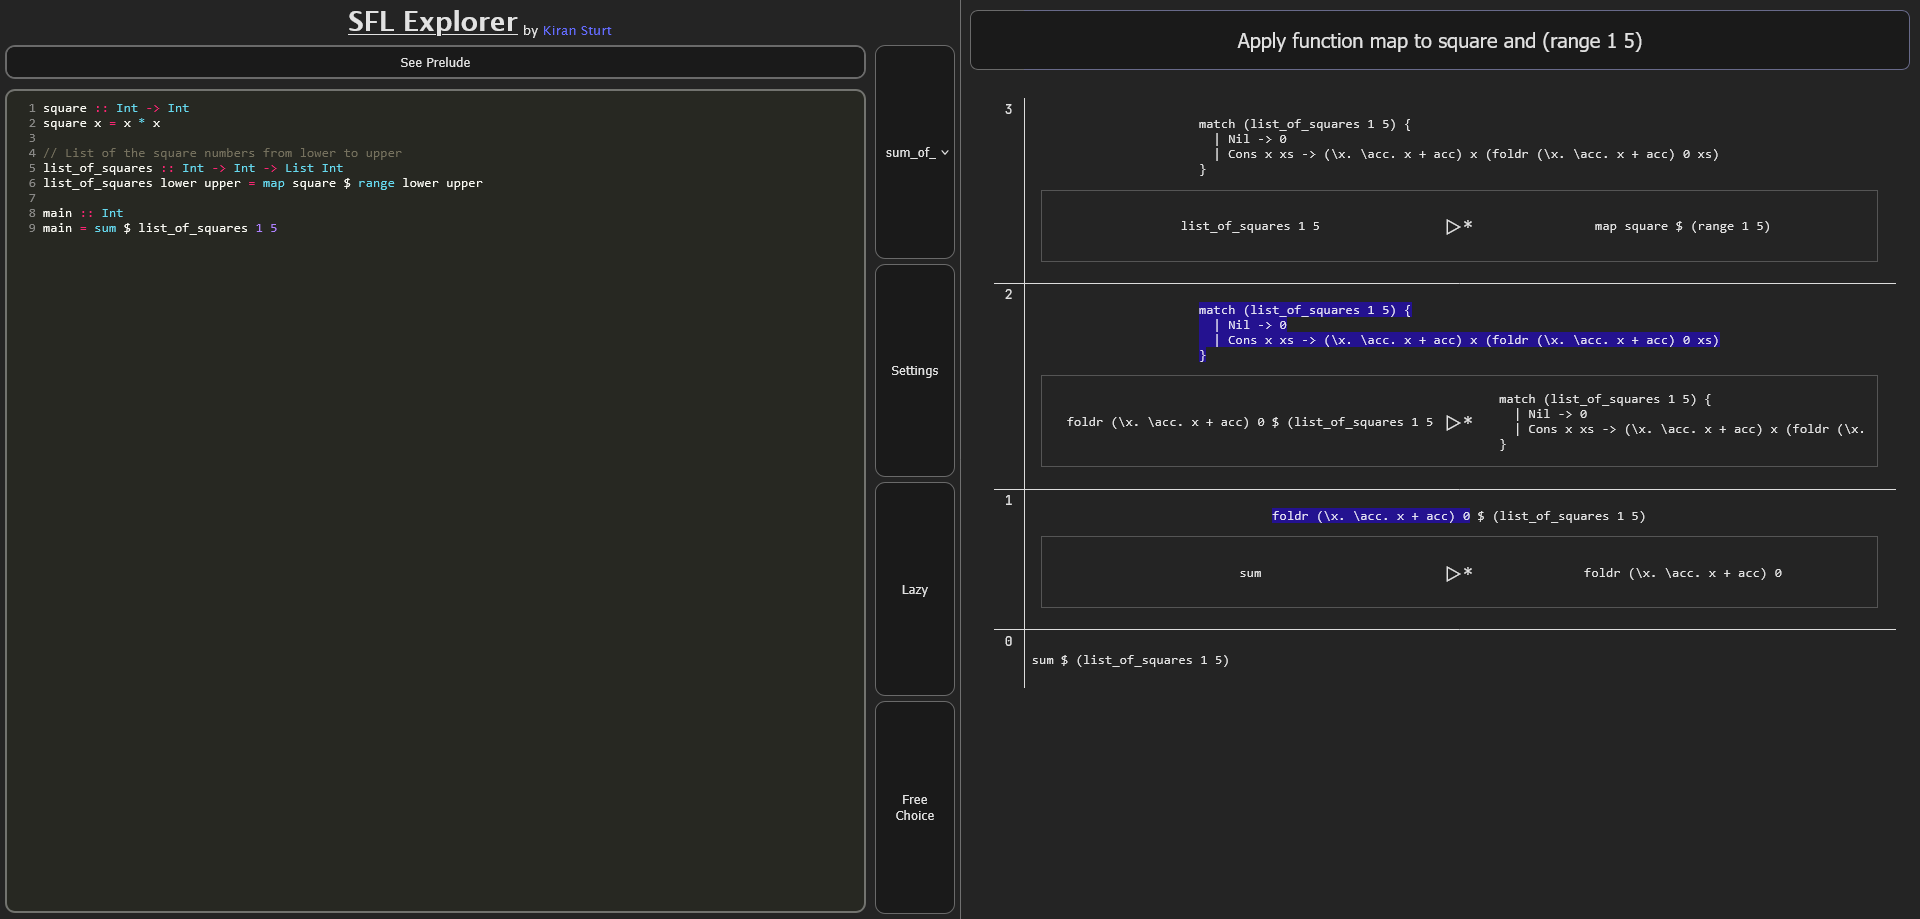
\includegraphics[width=\linewidth]{images/final_dark.png} 
    \captionsetup{justification=centering}
    \caption{The final product during lazy evaluation of the `sum of squares' sample program}
    \label{fig:screenshot_final_dark}
\end{figure}

\begin{figure}[h]
    \centering
    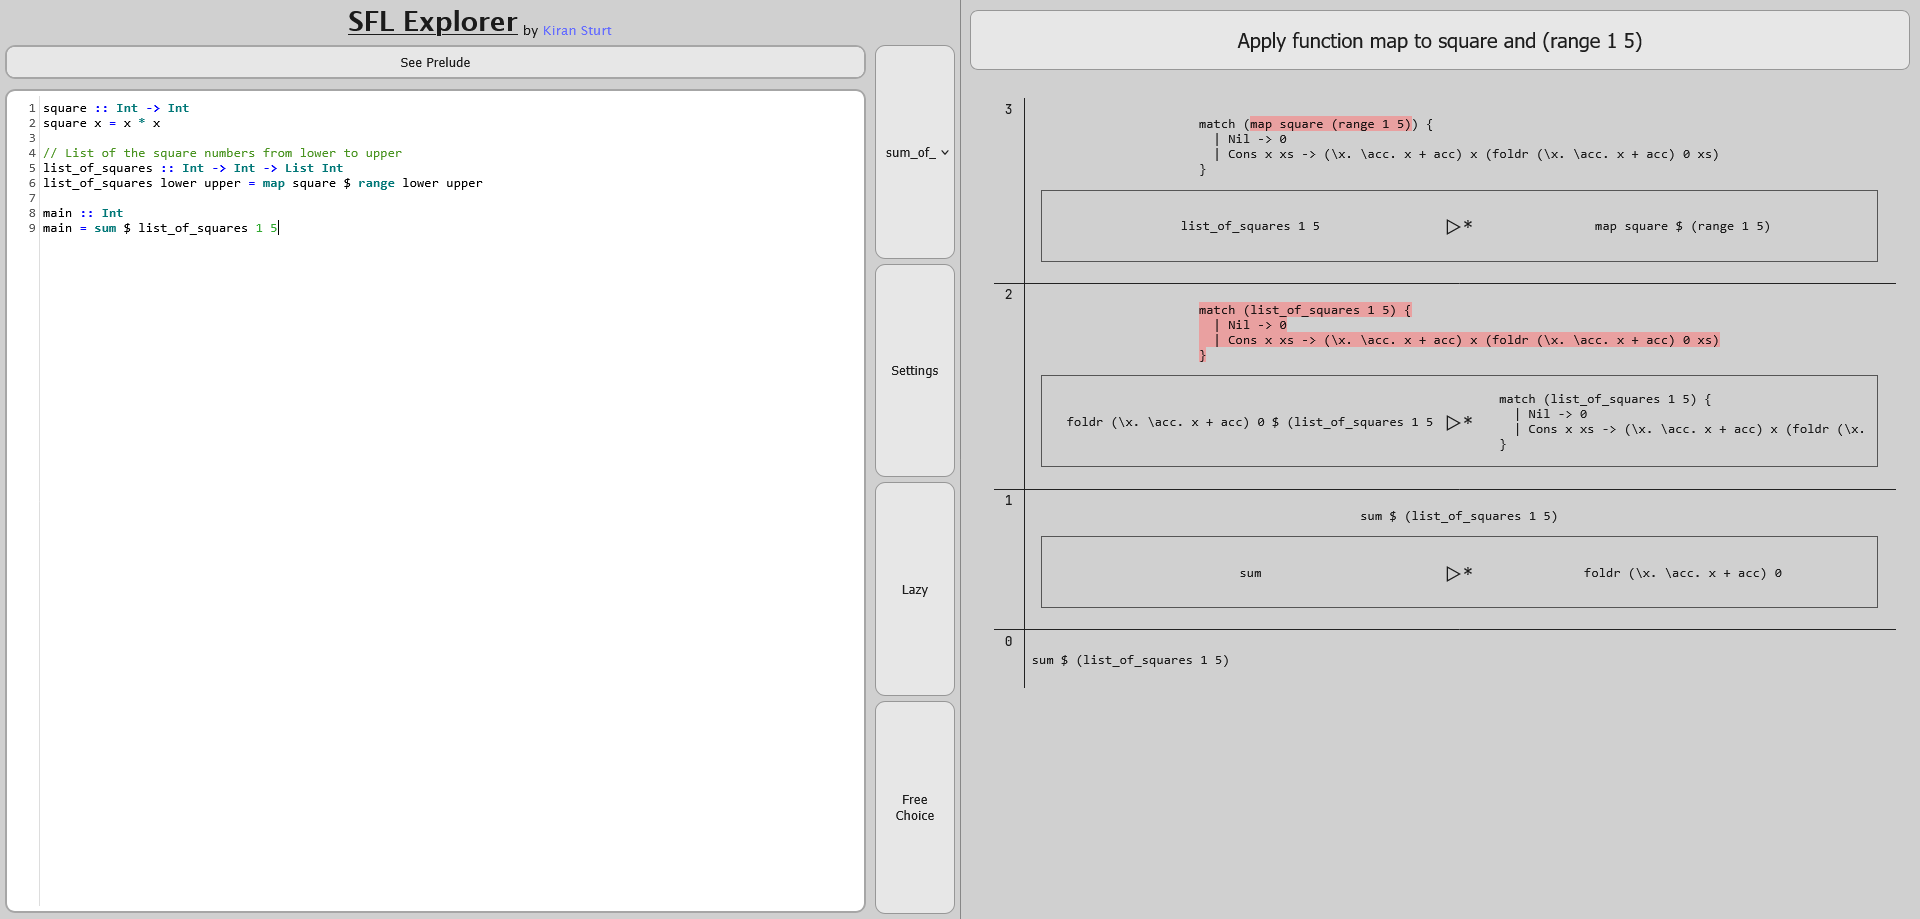
\includegraphics[width=\linewidth]{images/final_light.png} 
    \captionsetup{justification=centering}
    \caption{The final product during lazy evaluation of the `sum of squares' sample program in light mode}
    \label{fig:screenshot_final_light}
\end{figure}

\begin{figure}[h]
    \centering
    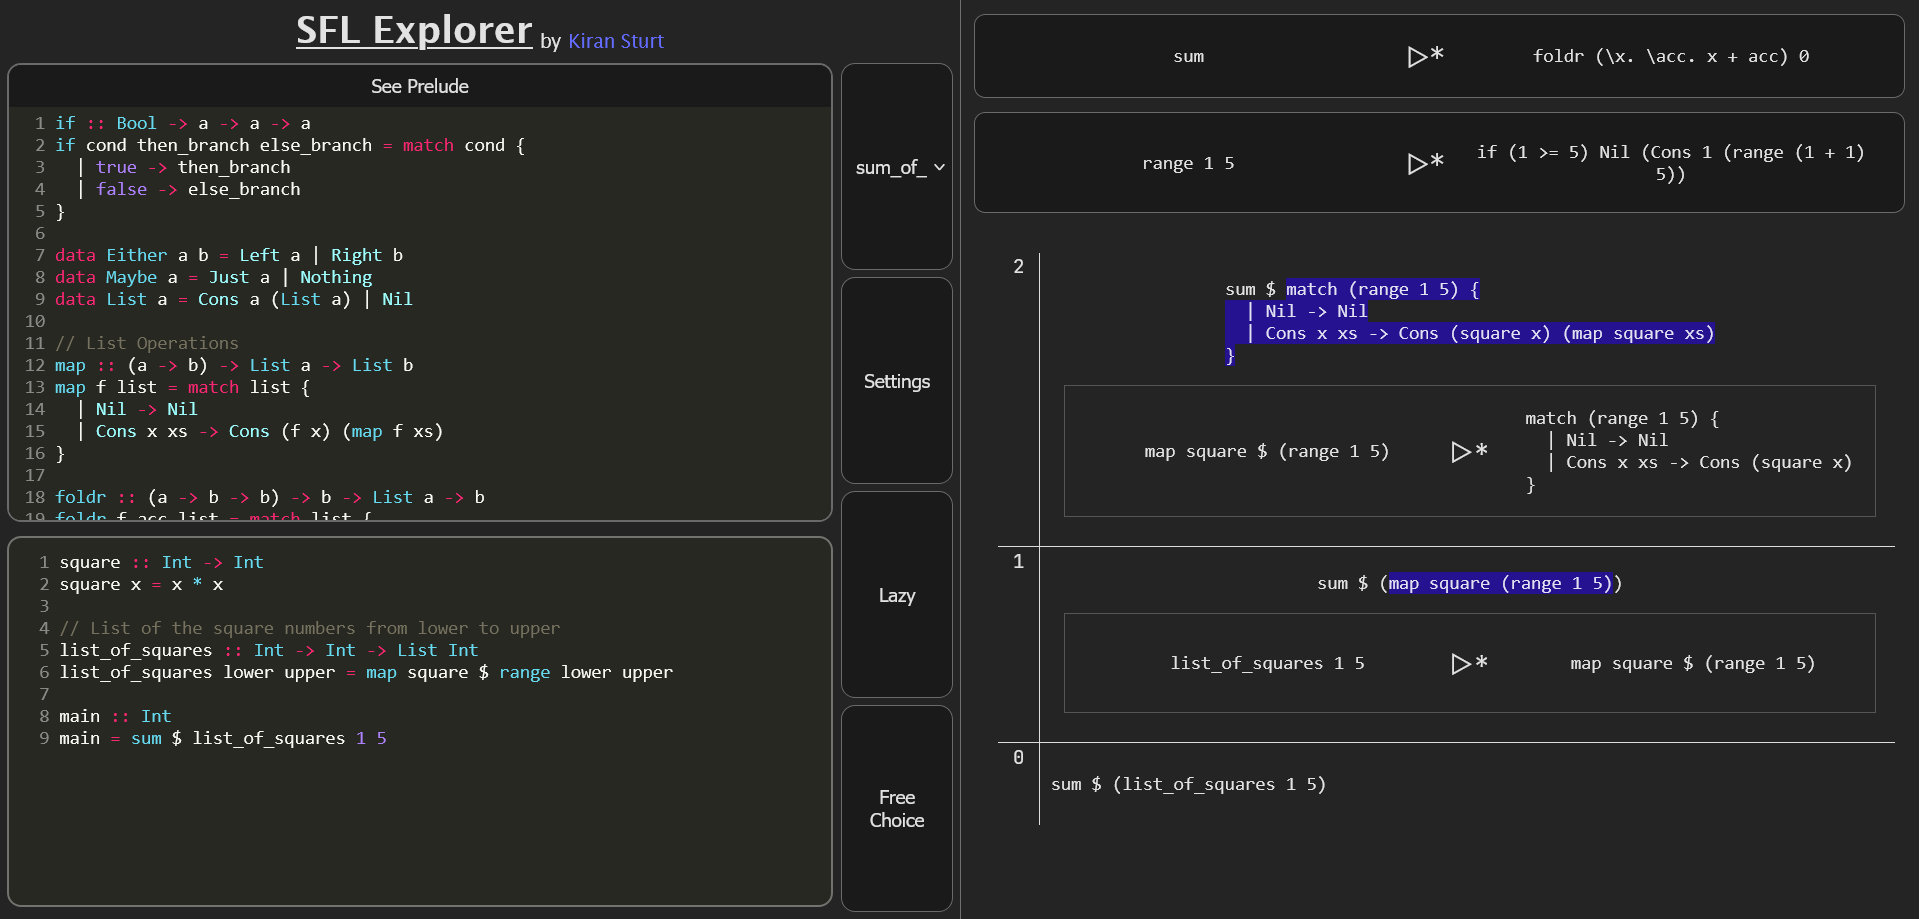
\includegraphics[width=\linewidth]{images/final_dark_prelude_free.png} 
    \captionsetup{justification=centering}
    \caption{The final product during free choice evaluation of the `sum of squares' sample program, with the prelude visible}
    \label{fig:screenshot_final_dark_prelude_free}
\end{figure}

\begin{figure}[h]
    \centering
    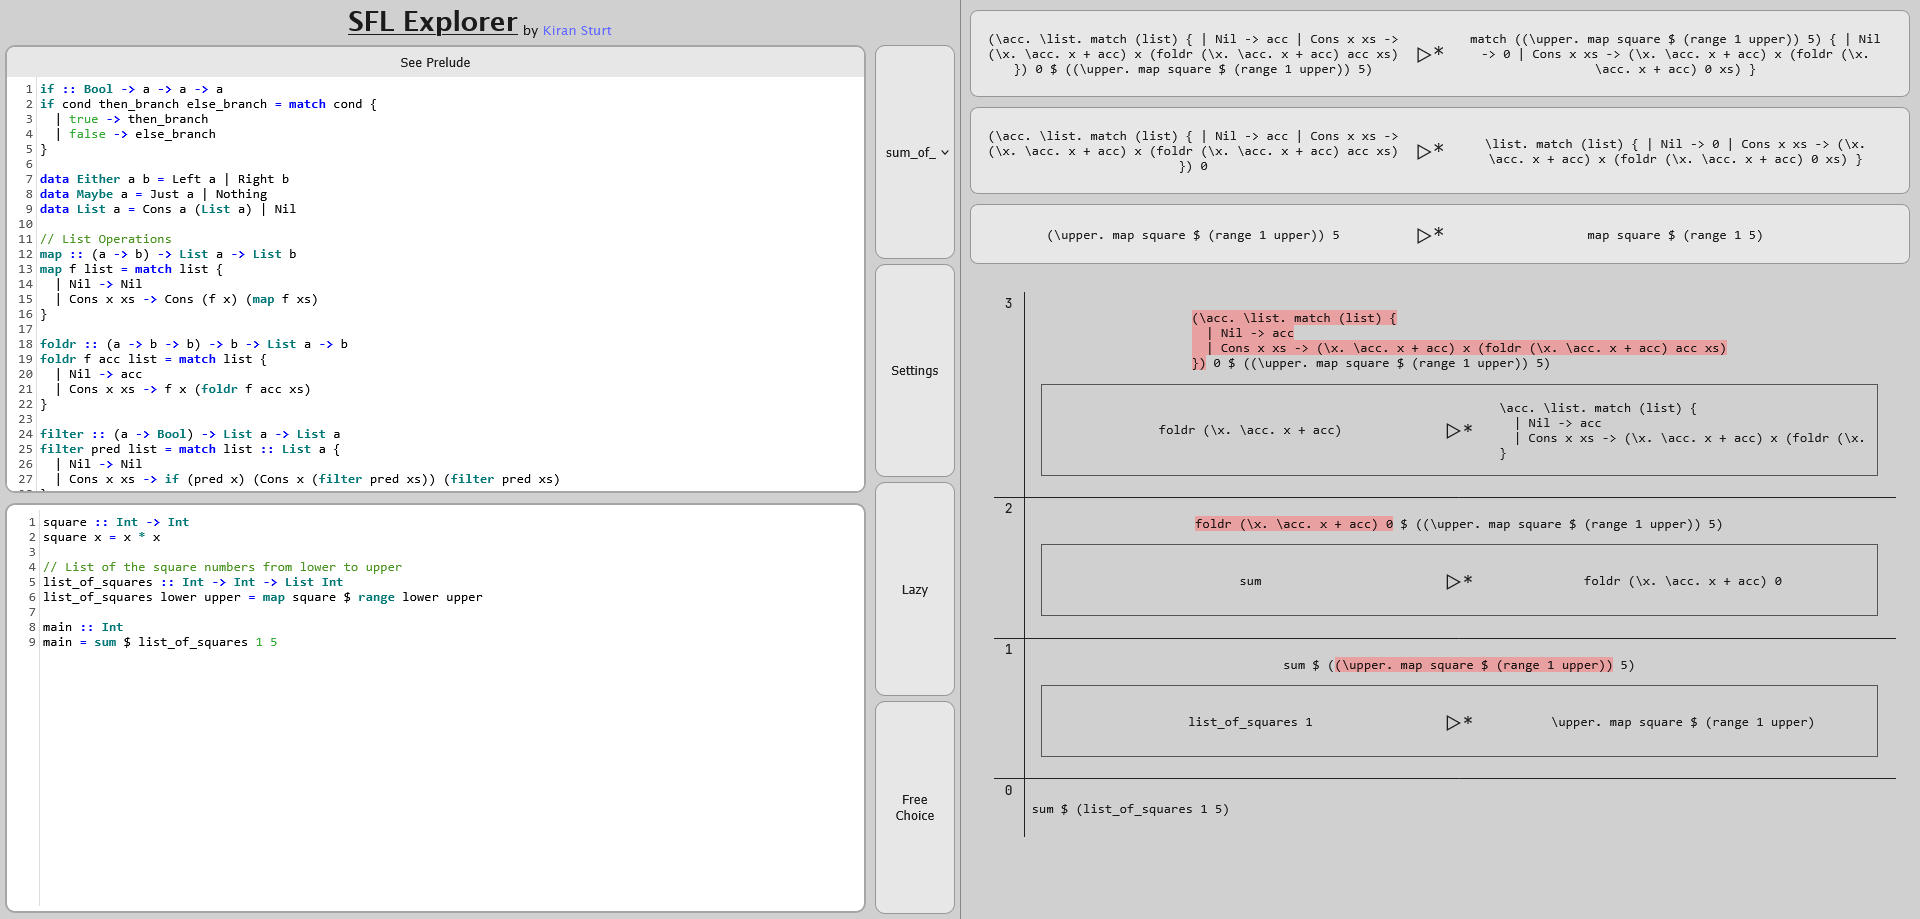
\includegraphics[width=\linewidth]{images/final_light_prelude_free.png} 
    \captionsetup{justification=centering}
    \caption{The final product during free choice evaluation of the `sum of squares' sample program, with the prelude visible in light mode}    
    \label{fig:screenshot_final_light_prelude_free}
\end{figure}

\chapter{Language Grammar}
\input{sections/lang_grammar}